\documentclass[a4paper, 8pt]{article}
\usepackage[latin1]{inputenc}
\usepackage[T1]{fontenc}
\usepackage[francais]{babel}
\usepackage{entete}
\usepackage{noitemsep}
\usepackage{euscript} 
\usepackage{amsmath,amssymb,amsfonts,amsthm}
\usepackage{graphicx,graphics,epsfig,subfigure,color}
\usepackage{url}
%\usepackage{algorithm2e}
\usepackage{multicol}
\usepackage{a4wide}
\usepackage{latexsym}
\usepackage{verbatim}
% \setlength{\textheight}{23.5cm}
% \setlength{\topmargin}{-1cm}
% \setlength{\textwidth}{155mm}
% \setlength{\oddsidemargin}{2mm}

\usepackage[paper=a4paper, bmargin=1.5cm, tmargin=1.5cm, lmargin=1.5cm, rmargin=1.5cm]{geometry} 
%\renewcommand{\baselinestretch}{0.85}

%\input{macroAlgo}
%\dontprintsemicolon

\setlength{\parindent}{0pt}  %%suppression indentation

%% DOC : https://xnau.com/work/wordpress-plugins/participants-database/participants-database-documentation/shortcodes-and-their-attributes/

\begin{document}
\selectlanguage{francais}
\author{D. Fourer}
\newcommand{\universityname}{IUT d'\'Evry Val d'Essonne}
\newcommand{\deptname}{D\'epartement TC (S3)}
\newcommand{\years}{2022-2023}

%------------------- TITRE -----------------------------------------
\date{Septembre 2021} 
\TDHead{\universityname}{\deptname}{R3.12 RCN3, \years}{\large TD6: base de donn\'ees avec Wordpress}
%\TDHead{DUT TC}{}{\large TIC3: Fonctions avanc\'ees d'un tableur}
%-------------------------------------------------------------------
%
\underline{Objectifs:} Manipulation d'une base de donn\'ees simple avec WordPress/Excel
%\vspace{-0.5cm}
%\section{} %%duree 30min, 1h maxi
%

\exost Depuis le tableau de bord de votre site, installez puis activez (si ce n'est pas d\'ej\`a fait) l'extension \textbf{``Participants Database''}:
\url{https://fourer.fr/Ens/2223/RCN3/participants-database.1.9.7.8.zip}.
Il s'agit d'un outil permettant de g\'erer une petite base de donn\'ees via Wordpress avec possibilit\'e d'import/export au format CSV
et saisie de formulaire en ligne.

\exost Ajout du formulaire permettant aux visiteurs d'ajouter des entr\'ees dans la base de donn\'ees:
\begin{enumerate}
 \item Cr\'eez une nouvelle \textbf{page} nomm\'ee ``R\'eunions''.
 \item Ajouter un texte introductif puis placez le \textit{shortcode} \verb?[pdb_signup]? en fin de page.
 \item Ajoutez cette page dans le \textbf{menu principal} du site dans la cat\'egorie ``Mes Activit\'es'' (cr\'e\'e au TP pr\'ec\'edent).
 \item Observez le r\'esultat obtenu en vous rendant sur la nouvelle page ainsi cr\'e\'ee.
\end{enumerate}

%% configuration
\exost Nous souhaitons maintenant configurer notre base de donn\'ees afin de permettre \`a des utilisateurs 
de s'inscrire \`a des r\'eunions.
%
\begin{enumerate}
 \item Ajoutez une nouvelle \textbf{page} nomm\'ee ``\'Edition Participant'' dans laquelle vous placerez le \textit{shortcode} \verb?[pdb_record]?
 \item Depuis le tableau de bord, allez dans ``configuration'' (Depuis le sous-menu de l'extension ``Participants Database'').
 \item Personnalisez le formulaire d'inscription (bouton du formulaire et mails de confirmation). Vous choisirez la page ``\'Edition Participant''
 depuis l'onglet ``R\'eglages du formulaire d\'etaill\'e''.
 \item Dans la rubrique ``G\'erer les champs de la base de donn\'ees'', modifiez les champs afin de conserver dans le formulaire uniquement:\\
 %
 \begin{tabular}{|l|l|}
 \hline
  Champ			& Caract\'eristiques\\
  \hline
  \hline
  {\bf Nom de famille}	& Champ de texte \\
  \hline
  {\bf Pr\'enom(s)}		& Champ de texte \\
  \hline
  Formation suivie	& boutons radio (choix parmi: FI1, FI2, FA1, FA2, autre) \\
  \hline
  Date de naissance 	& Champ de date \\
  \hline
  {\bf Jour pr\'ef\'er\'e}	& Cases \`a cocher \`a s\'election multiple (choix parmi les 7 jours de la semaine)\\
  \hline
  {\bf e-mail }		& Champ de texte \\
  \hline
 \end{tabular}
 \item Assurez vous que les cases CSV et inscription sont coch\'ees pour tous les champs sauf (adresse, city, state, country, zip, phone).
 \item Assurez vous que les champs nom, pr\'enom, jour pr\'ef\'er\'e et email sont obligatoires.
\end{enumerate}
%%

\exost Ajout d'une page en acc\`es prot\'eg\'e permettant de consulter la base de donn\'ee
\begin{enumerate}
 \item Cr\'eez une nouvelle \textbf{page} nomm\'ee ``Liste des inscrits'' que vous prot\'egerez par mot de passe (``visibilit\'e'')
 \item Ajouter un texte introductif puis placez le \textit{shortcode} \verb?[pdb_list]?.
 \item Ajoutez cette page dans le menu principal dans la cat\'egorie ``Mes activit\'es/R\'eunions'' (cf. Fig. \ref{fig:menu}).
 \item Visitez cette page et v\'erifiez que la page n'est pas accessible sans mot de passe.
 \item Choisissez les champs que vous souhaitez afficher via l'option ``Manage list columns''.
\end{enumerate}
\clearpage
\begin{figure}[!ht]
\begin{center}
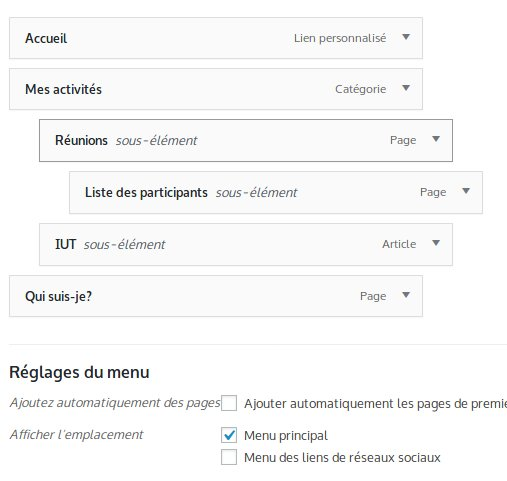
\includegraphics[height=5cm]{menu_wp.jpg} %width=0.7\textwidth, 
\end{center}
\caption{Structure du menu principal.}
\label{fig:menu}
\end{figure}



%% import/export CSV
\exost Testez le fonctionnement de votre formulaire d'enregistrement et r\'ecup\'erez les donn\'ees dans Excel:
\begin{enumerate}
 \item Remplissez plusieurs fois votre formulaire vous m\^eme (vous devrez recevoir un mail de confirmation contenant un lien d'\'edition \`a chaque fois).
 \item Invitez vos coll\`egues \`a visiter votre site puis \`a remplir le formulaire d'inscription.
 \item R\'ecup\'erez les donn\'ees enregistr\'ees en faisant un export CSV depuis la liste des participants (via le tableau de bord).
 \item Importez le fichier CSV dans Excel puis cr\'eez un tableau crois\'e dynamique permettant de compter le nombre total de r\'eponses par jour pr\'ef\'er\'e de la semaine.
 \item D\'eduisez le jour qui permettra de rassembler le plus de participants \`a votre prochaine r\'eunion.
\end{enumerate}

%\exost Plut\^ot qu'un mot de passe, cr\'eez un nouveau compte utilisateur puis donnez uniquement l'acc\`es

\end{document}

% End Of File

